\chapter{Metoda \emph{rotating calipers}\label{chap:calipers}}
Użyty w rozdziale~\ref{chap:diameter} algorytm można zobrazować jako
zestaw obracających się suwmiarek i jako ogólną metodę można
zastosować przy rozwiązywaniu innych problemów geometrycznych dla
wielokątów wypukłych; pozwala to na uzyskanie algorytmów działających
w czasie liniowym.

\section{Wyznaczanie średnicy}
W tej sekcji zostanie przedstawiony algorytm wyznaczania średnicy z
poprzedniego rozdziału z użyciem techniki \emph{rotating calipers}.

Niech $P = (p_0, p_2, \ldots, p_{n-1})$ będzie wielokątem wypukłym
oraz niech jego wierzchołki będą ponumerowane zgodnie z ruchem
wskazówek zegara. Algorytm z rozdziału~\ref{chap:diameter} znajduje
wszystkie pary antypodyczne, a następnie wybiera z nich najbardziej od
siebie oddalona parę wierzchołków, definiujących średnicę (na
podstawie twierdzenia~\ref{thm:yagbol}). Do znalezienia punktów
antypodycznych możemy użyć suwmiarki składającej się z dwóch
równoległych prostych wspierających. Rozważmy
rysunek~\ref{img:calipers1}. Jako początkową pozycję prostych
wspierających wyznaczmy prostą równoległą do osi $x$ przechodzącą
przez wierzchołek wielokąta $P$ położony najwyżej względem osi $y$
oraz równoległą do niej prostą przechodzącą przez wierzchołek
wielokąta $P$ położony najniżej względem osi $y$. Punkty $p_i$ i $p_j$
są pierwszą znalezioną parą antypodyczną. Aby znaleźć następną,
rozważmy kąty, które tworzy prosta wspierająca przechodząca przez
$p_i$ z krawędzią $(p_i, p_{i+1})$ oraz prosta wspierająca
przechodząca przez $p_j$ z krawędzią $(p_j, p_{j+1})$.  Jeżeli
$\angle{\theta_j} < \angle{\theta_i}$, to obracamy proste wspierające
o kąt $\theta_j$, w przeciwnym przypadku obracamy proste wspierające o
kąt $\theta_i$. Para $(p_{j+1}, p_i)$ staje się następną parą
antypodyczną. Proces powtarzamy do momentu, gdy proste wspierające
zamienią się miejscami, tj.\ gdy $p_j = p_{i_0}$ i $p_i = p_{j_0}$,
gdzie $p_{i_0}$ to wierzchołek styczny do początkowej pozycji
pierwszej prostej wspierającej, a $p_{j_0}$ to wierzchołek styczny do
początkowej pozycji drugiej prostej wspierającej.

\begin{figure}[htb]
  \centering
  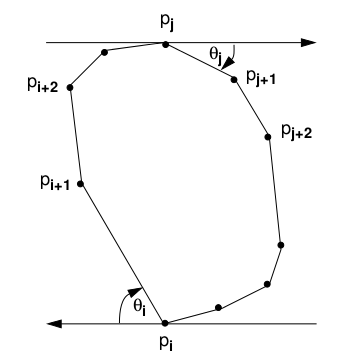
\includegraphics[scale=0.5]{img/calipers1}
  \caption{\label{img:calipers1} Wierzchołki $p_i$ i $p_j$ tworzą parę
    antypodalną.}
\end{figure}

\section{Najmniejszy prostokąt zawierający}
Problem najmniejszego prostokąta zawierającego zdefiniowany jest
następująco.

\begin{problem}[Najmniejszy prostokąt zawierający]
  Dla wielokąta wypukłego $P$ znaleźć najmniejszy prostokąt taki, żeby
  $P$ był w nim zawarty.
\end{problem}

Rozwiązanie tego problemu ma swoje zastosowanie m.\ in.\ w
przetwarzaniu obrazów, grach komputerowych i niektórych algorytmach
dotyczących optymalnego upakowania.

Algorytm z wykorzystaniem suwmiarek opiera się na następującym
twierdzeniu.

\begin{twierdzenie}[Freeman-Shapira 1975]
  Najmniejszy prostokąt zawierający wielokąt $P$ posiada bok
  współliniowy z bokiem $P$.
\end{twierdzenie}

Jako $L_s(p_i)$ będziemy oznaczać skierowaną prostą wspierającą
wielokąta w wierzchołku $p_i$ taką, że $P$ znajduje się po prawej
stronie prostej. Rozważmy rysunek~\ref{img:calipers2}. W pierwszym
kroku znajdujemy wierzchołki o minimalnych i maksymalnych
współrzędnych $x$ i $y$. Oznaczmy te wierzchołki jako $p_i$, $p_j$,
$p_k$, $p_l$. Niech para prostych $L_s(p_j)$ i $L_s(p_l)$ będzie
pierwszą suwmiarką, natomiast para $L_s(p_i)$ i $L_s(p_k)$
drugą. Analogicznie jak w algorytmie wyznaczającym średnicę, mamy tym
razem do rozważenia cztery kąty: $\angle{\theta_i}, \angle{\theta_j},
\angle{\theta_k}, \angle{\theta_l}$. Obróćmy teraz wszystkie cztery
proste wspierające o najmniejszy z nich. Wyznaczmy pole prostokąta
wyznaczonego przez punkty przecięć prostych wspierających $L_s(p_i),
L_s(p_j), L_s(p_k)$ i $L_s(p_l)$. Czynność tę powtarzamy z nowo
powstałymi kątami $\angle{\theta_i}, \angle{\theta_j},
\angle{\theta_k}, \angle{\theta_l}$ do czasu, gdy rozpatrzone zostaną
wszystkie możliwe prostokąty zawierające, tj.\ obydwie suwmiarki
wykonają pełny obrót wokół $P$. Ze wszystkich wyznaczonych w ten
sposób prostokątów wybieramy najmniejszy.

\begin{figure}[htb]
  \centering
  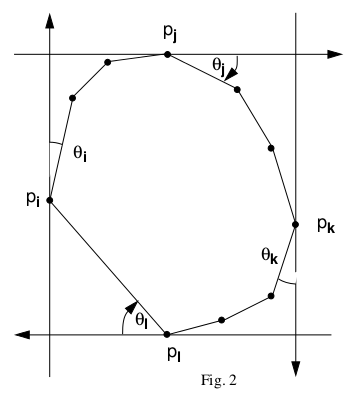
\includegraphics[scale=0.5]{img/calipers2}
  \caption{\label{img:calipers2} Pary wierzchołków $(p_i, p_k)$ i
    $(p_j, p_l)$ są parami antypodycznymi.}
\end{figure}

\section{Największa odległość\label{sec:max_dist}}
\begin{problem}
  Niech $P = (p_1, p_2, \ldots, p_n)$ oraz $Q = (q_1, q_2, \ldots,
  q_m)$ będą wielokątami wypukłymi. Największą odległość między $P$ i
  $Q$ oznaczamy jako $d_{\max}(P, Q)$ i definiujemy
  jako: $$d_{\max}(P, Q) := \max{\{ d(p_i, q_j) \mid i = 1, 2, \ldots,
    n; j = 1, 2, \ldots, m \}},$$ gdzie $d(p_i, q_j)$ oznacza
  odległość euklidesową pomiędzy $p_i$ i $q_j$.
\end{problem}

Należy zauważyć, że największa odległość między dwoma wielokątami
wypukłymi nie musi być równa średnicy otoczki wypukłej $P \cup Q$
(rysunek~\ref{fig:maxdist}), więc nie możemy wykorzystać algorytmu
wyznaczającego średnicę do rozwiązania tego problemu.

\begin{figure}[htb]
  \centering
  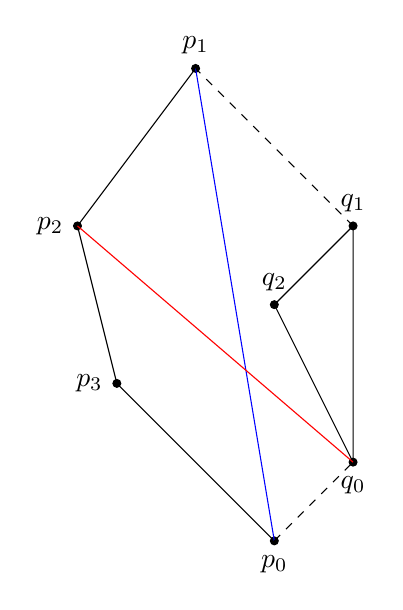
\begin{tikzpicture}
      \coordinate (p1) at (3,5);
      \coordinate (p2) at (1.5,3);
      \coordinate (p3) at (2,1);
      \coordinate (p0) at (4,-1);

      \draw (p1) -- (p2) -- (p3) -- (p0);

      \node [anchor=center,circle,draw,fill,inner
      sep=1pt,label={below:$p_0$}] at (p0) {};

      \node [anchor=center,circle,draw,fill,inner
      sep=1pt,label={above:$p_1$}] at (p1) {};

      \node [anchor=center,circle,draw,fill,inner
      sep=1pt,label={left:$p_2$}] at (p2) {};

      \node [anchor=center,circle,draw,fill,inner
      sep=1pt,label={left:$p_3$}] at (p3) {};

      \coordinate (q0) at (5,0);
      \coordinate (q1) at (5,3);
      \coordinate (q2) at (4,2);

      \node [anchor=center,circle,draw,fill,inner
      sep=1pt,label={below:$q_0$}] at (q0) {};

      \node [anchor=center,circle,draw,fill,inner
      sep=1pt,label={above:$q_1$}] at (q1) {};

      \node [anchor=center,circle,draw,fill,inner
      sep=1pt,label={above:$q_2$}] at (q2) {};

      \draw (q0) -- (q1) -- (q2) -- cycle;

      \draw [blue] (p0) -- (p1);

      \draw [red] (p2) -- (q0);

      \draw [dashed] (q1) -- (p1);
      \draw [dashed] (p0) -- (q0);
  \end{tikzpicture}
  \caption{\label{fig:maxdist} Odcinek $(p_0, p_1)$ jest średnicą otoczki
    wypukłej $P \cup Q$, natomiast odcinek $(p_2, q_0)$ jest największą
    odległością między tymi wielokątami.}
\end{figure}

Rozważmy rysunek~\ref{img:calipers3}. W pierwszym kroku znajdujemy dwa
punkty, z których jeden $p_i$ należy do $P$, a drugi $q_j$ do $Q$, tak
aby proste wspierające $L_s(p_i)$ i $L_s(p_j)$ były równoległe. Możemy
na przykład wybrać punkty o skrajnym położeniu względem osi $y$. Niech
$L_s(p_i)$ i $L_s(q_j)$ będą prostymi skierowanymi w przeciwnych
kierunkach. Utworzone w ten sposób proste wspierające tworzą kąt
$\angle{\theta_i}$ z krawędzią $(p_i, p_{i+1}) \in P$ oraz kąt
$\angle{\phi_j}$ z krawędzią $(q_j, q_{j+1}) \in Q$. Wyznaczamy i
zapamiętujemy odległość między $p_i$ i $q_j$. Wybieramy mniejszy z
kątów $\phi_j$ i $\theta_i$, a następnie obracamy obydwie proste
wspierające o ten kąt. Proces powtarzamy do czasu, gdy proste
wspierające zamienią się początkowymi pozycjami. W ostatnim kroku
wybieramy największą z wyznaczonych odległości między punktami.

\begin{figure}[htb]
  \centering
  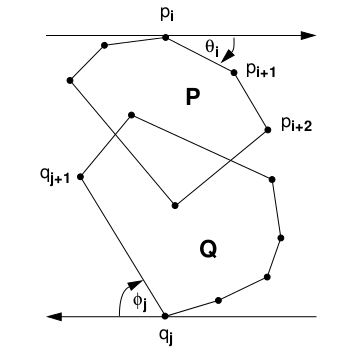
\includegraphics[scale=0.5]{img/calipers3}
  \caption{\label{img:calipers3} Para wierzchołków $(p_i, q_j)$ jest
    parą antypodalną między wielokątami $P$~i~$Q$.}
\end{figure}

\section{Łączenie otoczek wypukłych}
\begin{problem}
  Dla $CH(P)$ i $CH(Q)$ będącymi otoczkami wypukłymi zbiorów $P$ i
  $Q$ znaleźć otoczkę wypukłą $CH(CH(P) \cup CH(Q))$.
\end{problem}

W algorytmach typu \emph{dziel i zwyciężaj} wyznaczających otoczkę
wypukłą zbioru punktów końcowym etapem jest łączenie otoczek
uzyskanych w poprzednim kroku, uzyskując w ten sposób coraz większe
otoczki, aż do uzyskania otoczki wypukłej całego zbioru. Jeśli łącznie
zostałoby przeprowadzone w czasie liniowym, złożoność czasowa całego
algorytmu w najlepszym przypadku będzie
liniowo-logarytmiczna~\cite{Graham72}.

\begin{figure}[htb]
  \centering
  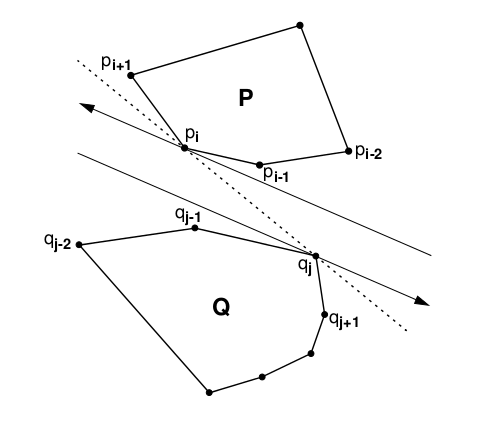
\includegraphics[scale=0.5]{img/calipers4}
  \caption{\label{img:calipers4} Wierzchołki $p_i$ i $q_j$ tworzą parę
    kopodalną.}
\end{figure}

Rozważmy dwa wielokąty wypukłe $P = (p_1, \ldots, p_n)$ i $Q = (q_1,
\ldots, q_n)$, gdzie wierzchołki $P$ i $Q$ są numerowane zgodnie z
kierunkiem ruchu wskazówek zegara, będącymi otoczkami wypukłymi
pewnych zbiorów punktów (rysunek~\ref{img:calipers4}). W tym przypadku
wyznaczenie otoczki wypukłej obydwu wielokątów wymaga znalezienia
dwóch par wierzchołków $(p_i, p_j)$, $(q_k, q_l)$ takich, że krawędzie
$(p_i, q_k)$ i $(p_j, q_l)$ wraz z łańcuchami wypukłymi $(p_i,
p_{i+1}, \ldots, p_j)$ i $(q_k, q_{k+1}, \ldots, q_l)$ tworzą $CH(P
\cup Q)$. Krawędzie $(p_i, q_k)$ i $(p_j, q_l)$ będziemy nazywać
\emph{mostami}, a wierzchołki tworzące most będziemy nazywać
\emph{punktami mostu}. Ponadto mówimy, że para punktów $p \in P$ i $q
\in Q$ jest \emph{parą kopodoalną między $P$ i $Q$}, jeżeli można
skonstruować równoległe proste wspierające styczne do wierzchołków $p$
i $q$ odpowiednio.

Algorytm wykorzystujący suwmiarki do wyznaczania mostów opiera się na
następującym twierdzeniu~\cite{Toussaint83}.

\begin{twierdzenie}[Toussaint 1983]
\label{thm:bridge}
Dwa wierzchołki $p_i \in P$ i $q_j \in Q$ są punktami mostu wtedy i
tylko wtedy, gdy tworzą parę kopodalną i wierzchołki $p_{i-1},
p_{i+1}, q_{j-1}$, $ q_{j+1}$ leżą po tej samej stronie prostej
$L(p_i, q_j)$.
\end{twierdzenie}

Po wyznaczeniu pozycji suwmiarek, analogicznie jak w algorytmie
\ref{sec:max_dist}, skierowanych w przeciwnych kierunkach, zaczynamy
obracać je wokół wielokątów. Podobnie jak w poprzednich problemach
rozważamy kąt, jaki tworzy skierowana prosta wspierająca wielokąta $P$
w punkcie $p_i$ z krawędzią $(p_{i+1}, p_{i+2})$ oraz prosta
wspierająca wielokąta $Q$ z krawędzią $(q_{j+1}, q_{j+2})$. Obydwie
suwmiarki obracamy o mniejszy z tych kątów. Przed każdym kolejnym
obrotem sprawdzamy, czy aktualna para wierzchołków $(p_i, q_j)$
spełnia warunek zawarty w twierdzeniu~\ref{thm:bridge}. Ponieważ przy
każdym obrocie suwmiarek generowana jest nowa para kopodalna,
pozostaje sprawdzić, czy wierzchołki $p_{i-1}, p_{i+1}, q_{j-1},
q_{j+1}$ leżą po tej samej stronie prostej $L(p_i, q_j)$. Algorytm
znajdowania mostów w przypadku łączenia otoczek wypukłych można
zakończyć po znalezieniu obydwu mostów.

Niech liczba wierzchołków $P$ wynosi $n$, a liczba wierzchołków $Q$
wynosi $m$. Par kopodalnych jest mniej niż $n + m$. Sprawdzenie, czy
para kopodalna jest mostem, odpobywa się w czasie $O(1)$, stąd
złożoność czasowa algorytmu wyznaczającego mosty jest rzędu $O(n +
m)$.

%%% Local Variables:
%%% mode: latex
%%% TeX-master: "masterthesis"
%%% TeX-engine: xetex
%%% End:
